\section{DC motoren}
Dette appendix beskæftiger sig med bestemmelsen af motorparametrene.
\subsection{DC Motor karakteristik}
DC Motoren kan modelleres efter diagrammet på figur \ref{fig:DCmotor}. \todo[]{Kredsløbsdiagram skal tegnes i tikz}

\begin{figure}[!th]
\centering
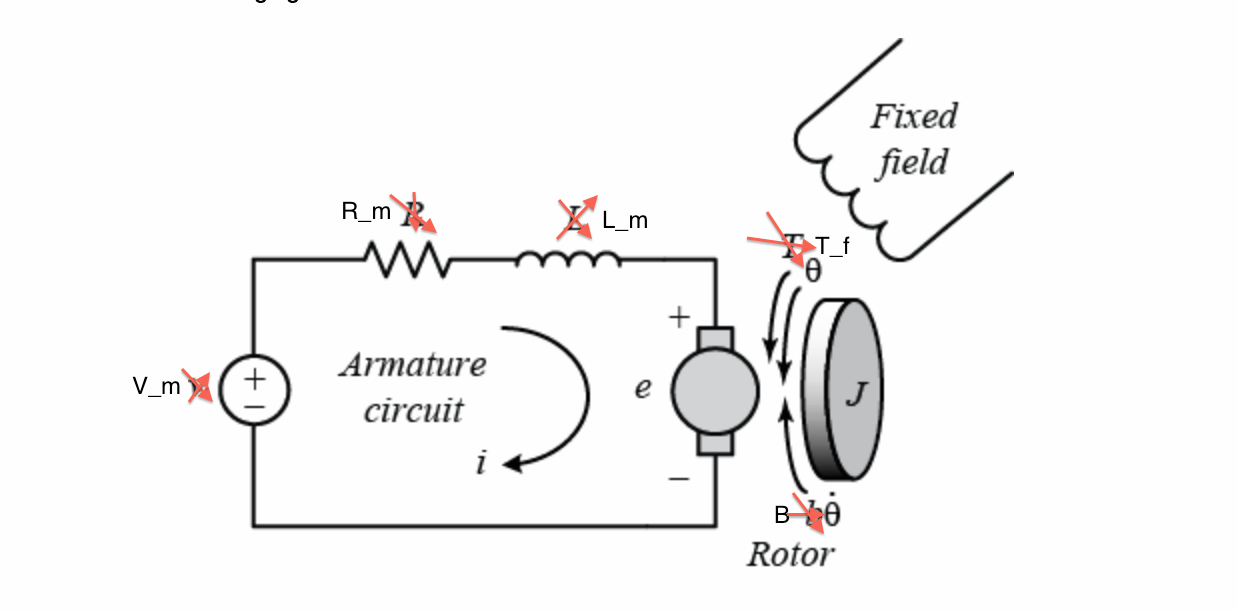
\includegraphics[width=0.7\textwidth]{./graphics/Mangleratblivetegnet}
%\begin{tikzpicture}[scale=2]
%\include*{./graphics/}
%\end{tikzpicture}
\caption[DC motor]{Diagram over fysiske komponenter i DC motoren.}
\label{fig:DCmotor}
\end{figure}
Ligningen for \(V_m\) er givet ved ligning \ref{eq:Vm_transient0}, \citep{DCmotormodel}.
\begin{equation}
	V_m(t)=L_m \cdot \frac{\mathrm d}{\mathrm d t} \big( i_m(t) \big)+R_m \cdot i_m(t) + V_{EMF}(t)
	\label{eq:Vm_transient0} 
 \end{equation}
Den modelektromotoriske kraft, \(V_{EMF}\) er givet ved ligning \ref{eq:VEMF}.
\begin{equation}
	V_{EMF}(t) = K_b \cdot \omega(t)
	\label{eq:VEMF}
\end{equation}
Med ligning \ref{eq:VEMF} kan ligning \ref{eq:Vm_transient0} omskrives til ligning \ref{eq:Vm_transient1}.
\begin{equation}
	V_m(t)=L_m \cdot \frac{\mathrm d}{\mathrm d t} \big( i_m(t) \big)+R_m \cdot i_m(t) +K_b \cdot \omega(t)
	\label{eq:Vm_transient1} 
 \end{equation}

Kraftmomentet kan udtrykkes som funktion af strømmen, som i ligning \ref{eq:Tm_im}.
\begin{equation}
	T_m(t)=K_t\cdot{i_m(t)}
	\label{eq:Tm_im} 
 \end{equation}
Samtidig kan kraftmomentet, som motoren producerer, udtrykkes som multiplikationen af inertimoment og vinkelacceleration.
Det inertimoment, der leveres til belastningen vil være kraftmomentet fra motoren fratrukket friktionen.
Friktionen antages til disse beregninger at være viskøs, dvs. proportional med vinkelhastigheden.
Kraftmomentet kan altså udtrykkes ved ligning \ref{eq:Tm_leveret}
\begin{equation}
	T_m(t)=J\cdot\frac{\mathrm d}{\mathrm d t} \big(\omega(t) \big)+B\cdot\omega(t)
	\label{eq:Tm_leveret} 
 \end{equation}

Proportionalitetskonstanterne \(K_b\) og \(K_t\) har i SI-enheder samme numeriske værdi, \citep[Physical setup]{matlabdcmodel}.

\subsection{Eksperiment 1}
\label{ss:eksperiment1}
\subsubsection{Formål}
Bestemmelse af motorens ækvivalente resistans, \(R_m\).
\subsubsection{Teori}
Forhindres motoren i at rotere, vil vinkelhastigheden være nul.
Hvis man påfører motoren en DC-spænding \(V_m\),
og venter til motorens respons har nået steady-state,
så vil strømmen igennem motoren være konstant.
Her vil ligning \ref{eq:Vm_transient1} kunne omskrives til ligning \ref{eq:resistans_E1}.
\begin{equation}
	V_m=R_m \cdot i_m
	\label{eq:resistans_E1} 
 \end{equation}
Målinger af sammenhørende steady-state værdier for strøm \(i_m\) og spænding \(V_m\)
kan altså bruges til bestemmelse af den ækvivalente resistans \(R_m\).
\subsubsection{Fremgangsmåde}
Motoren låses fast vha. en skiftenøgle og påføres en lav spænding.
Efter nogle sekunder, når transientresponsen er væk,
måles spændingen over og strømmen igennem motoren med multimetre.
Værdierne noteres, og forsøget gentages ved andre spændinger.

De anvendte multimetre er af typen TTi 1604.
\subsubsection{Måleresultater}
I tabel \ref{tb:resistans} findes målingerne af strøm og spænding.
\begin{figure}[th!]
	\centering
	%\begin{tabular}{r|r}
%$V_m$ [V]&$i_m$ [A]\\\hline
%0,509&0,094 \\ %0,5093&0,094 \\
%0,883&0,172 \\ %0,8833&0,172
%1,481&0,297 \\ %1,4809&0,297 
%1,940&0,391 \\ %1,9404&0,391
%2,345&0,470 \\ %2,3448&0,470
%2,788&0,555 \\ %2,7879&0,555
%3,182&0,638 \\ %3,1823&0,638
%3,465&0,664 \\ %3,4652&0,664
%3,835&0,746 \\ %3,8346&0,746
%4,067&0,765 \\ % 4,067&0,765
%4,292&0,830 \\ %4,292&0,830 
%\end{tabular}


\begin{tabular}{r|r|r|r|r|r|r|r|r|r|r|r}
$V_m$ [V]&0,509&0,883&1,1481&1,940&2,345&2,788&3,182&3,465&3,835& 4,067&4,292\\\hline
$i_m$ [A]&0,094&0,172&0,297 &0,391&0,470&0,555&0,638&0,664&0,746&0,765&0,830
\end{tabular}
	\captionsetup{type=table}
	\caption[Sammenhørende værdier af DC spænding og strøm]
			{Sammenhørende værdier af DC spænding over og strøm gennem rotationslåst motor.}
	\label{tb:resistans}
\end{figure}
\subsubsection{Databehandling}
Den målte strøm-spændingskarakteristik for DC-motoren er indtegnet på figur \ref{fig:resistans0}.
\begin{figure}[th!]
	\centering
	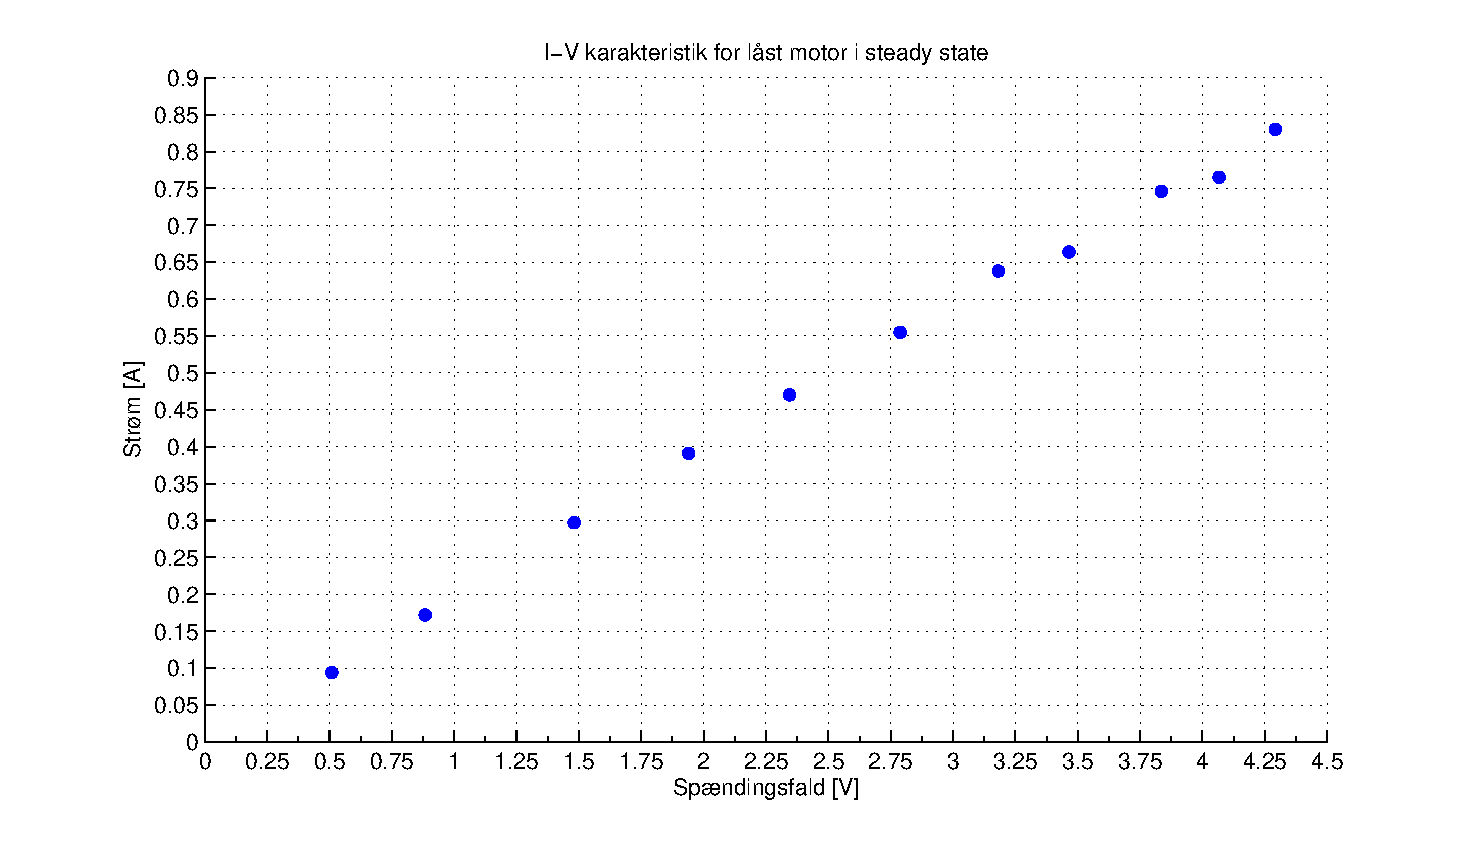
\includegraphics[width=1\textwidth]{./graphics/resistans1.eps}
	\caption[Strøm-spændingskarakteristik for rotationslåst DC-motor]{Strøm-spændingskarakteristik for rotationslåst DC-motor ved steady-state.}
	\label{fig:resistans0}
\end{figure}
Som det ses på figur \ref{fig:resistans0} er sammenhængen mellem strøm og spænding
tilnærmelsesvis lineær, og en lineær regression på dataene vil altså give en tilnærmet værdi for \(R_m\).
\(R_m\) er ved lineær regression beregnet til 5,215 \([\Omega]\).\\
Den mindste effektafsættelse i motoren var 48 [mW].

\subsubsection{Diskussion}
Da sammenhængen mellem strøm og spænding i målingerne er tilnærmelsesvis lineær,
vurderes den fundne værdi for \(R_m\) at være meget nøjagtig,
om ikke andet, så for effektafsættelser i motoren på mindst 48 [mW].

\subsubsection{Konklusion}
Motorens ækvivalente resistans, \(R_m\) er vha. sammenhørende målinger af strøm og spænding
for en rotationslåst motor, ved effektafsættelser i motoren på 48 [mW] og højere,
blevet bestemt til 5,215 \([\Omega]\).

\subsection{Eksperiment 2}
\label{ss:eksperiment2}
\subsubsection{Formål}
Bestemmelse af motorens ækvivalente induktans, \(L_m\).
Der er benyttet tre forskellige metoder til bestemmelsen af induktansen.
Metode 1 tager udgangspunkt i tidskonstanten for et RL-kredsløb,
mens metode 2 tager udgangspunkt i faseforskellen mellem forskellige komplekse impedanser i serie.
Metode 3 benytter et LCR-meter, som er et måleapparat der kan måle en passiv komponents impedans, til bestemmelsen af induktansen.
\subsubsection{Teori}
\paragraph{Metode 1\\}
Forhindres motoren i at rotere, vil vinkelhastigheden som beskrevet i afsnit \ref{ss:eksperiment1} være nul.
Ved denne metode er vi interesseret i systemets transientrespons, hvor strømmen \(i_m\) ikke er konstant.
Forbindes en modstand \(R_s\) i serie med DC-motoren som vist på figur \ref{fig:eksperiment2metode1} vil der være tale om et RL-kredsløb, med en tidskonstant \(\tau\) givet ved ligning \ref{eq:rltimeconstant}.

\begin{figure}[!th]
\centering
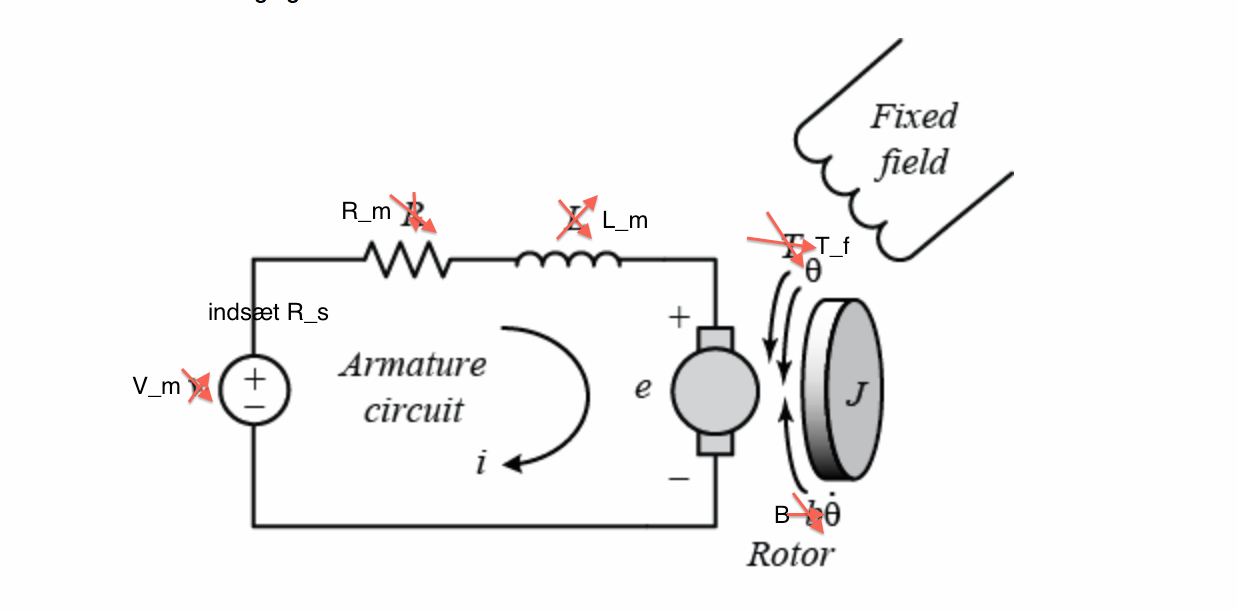
\includegraphics[width=0.1\textwidth]{./graphics/Mangleratblivetegnet2}
%\begin{tikzpicture}[scale=2]
%\include*{./graphics/}
%\end{tikzpicture}
\caption[]{MANGLER AT BLIVE TENGET}
\label{fig:eksperiment2metode1}
\end{figure}


Transientresponsen for alle strømme og spændingsfald i kredsløbet har denne tidskonstant.

\begin{equation}
	\tau=\frac{L_m}{R_m+R_s}
	\label{eq:rltimeconstant} 
 \end{equation}
Tidskonstanten er et mål for tiden det tager systemet at opnå \textbf{ca.??} 63,2 \% af slutværdien. For en (eksponentielt) aftagende kurve med tidskonstanten \(\tau\) kan tidskonstanten aflæses som
tidsforskellen mellem to niveauer \(V_0\) og \(V_1\), hvor \(V_1\) er ca. 36,8 \% af \(V_0\).

Ved omskrivning af ligning \ref{eq:rltimeconstant} kan induktansen altså bestemmes vha. ligning \ref{eq:induktans0}.
\begin{equation}
	L_m=\tau\cdot(R_m+R_s)
	\label{eq:induktans0} 
 \end{equation}
\paragraph{Metode 2\\}
Forhindres motoren i at rotere, vil vinkelhastigheden som beskrevet i afsnit \ref{ss:eksperiment1} være nul.
Ved denne metode er vi interesseret i systemets steady-state respons.
Forbindes en modstand \(R_{s1}\) i serie med DC-motoren som vist på figur ref{fig:eksperiment2metode2}
vil impedansen \(\mathbf{Z_m}\) af DC-motoren være givet ved ligning \ref{eq:zm_0}.

\begin{figure}[!th]
\centering
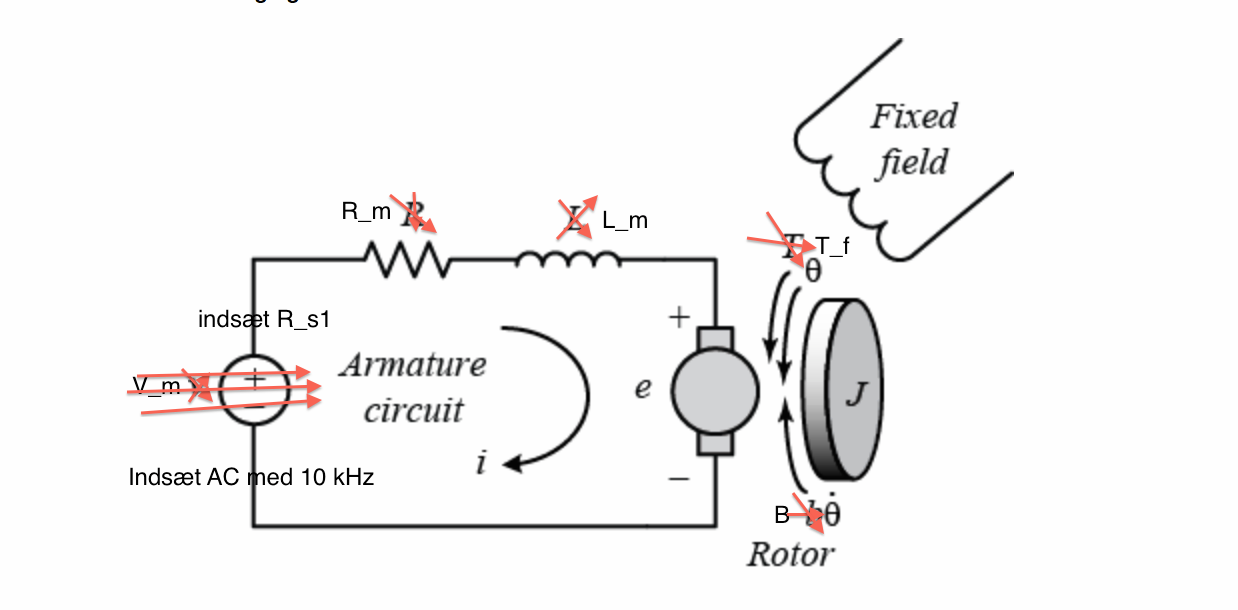
\includegraphics[width=0.1\textwidth]{./graphics/Mangleratblivetegnet3}
%\begin{tikzpicture}[scale=2]
%\include*{./graphics/}
%\end{tikzpicture}
\caption[]{MANGLER AT BLIVE TENGET - Indsæt kredsløbsdiagram med Rs1 og AC-forsyning med DC offset}
\label{fig:eksperiment2metode2}
\end{figure}


\begin{equation}
	\mathbf{Z_m}=R_{s1}\cdot\frac{\mathbf{V_1}-\mathbf{V_2}}{\mathbf{V_2}}
			=R_{s1}\cdot\left(\frac{\mathbf{V_1}}{\mathbf{V_2}}-1\right)
			=R_{s1}\cdot\left(\frac{A_1}{A_2}\cdot{e}^{\phi}-1\right)
	\label{eq:zm_0} 
 \end{equation}
Bemærk at spændingsfaldene noteres med fed skrift for at indikere at her er tale om phasors,
at \(A_1\) og \(A_2\) angiver amplituderne af \(\mathbf{V_1}\) og \(\mathbf{V_2}\),
samt at \(\phi=\phi_1-\phi_2\) angiver faseforskellen mellem de to signaler.
Denne faseforskel kan også udtrykkes ved tidsforsinkelsen \(\Delta{t}\) ganget med vinkelfrekvensen \(\omega\).
Ligning \ref{eq:zm_1} angiver impedansen på rektangulær form.
\begin{equation}
	\mathbf{Z_m}=R_{s1}\cdot\left(\frac{A_1}{A_2}\cdot{\cos (\phi)}-1\right)	%Realdel
	+\mathbf{j}\cdot{R_{s1}}\cdot\frac{A_1}{A_2}\cdot\sin(\phi)	%Imaginærdel
	\label{eq:zm_1} 
 \end{equation}
Samtidig vides det, at den rotationslåse motors impedans består af resistansen \(R_m\) samt
reaktansen \(X_m\), hvor \(X_m\) er reaktansen for en spole, altså \(\omega\cdot{L_m}\).
Motorens impedans kan altså også beskrives ved ligning \ref{eq:zm_2}, hvor \(\mathbf{j}\) er den imaginære enhed.
\begin{equation}
	\mathbf{Z_m}=R_m+\mathbf{j}\cdot\omega\cdot{L_m}
	\label{eq:zm_2} 
 \end{equation}
Sættes ligningerne \ref{eq:zm_1} og \ref{eq:zm_2} lig med hinanden
kan man altså udtrykke resistansen \(R_m\) og induktansen \(L_m\) som funktioner
af faseforskellen på \(\mathbf{V_1}\) og \(\mathbf{V_2}\),
hvilket giver ligningerne \ref{eq:Rm_0} og \ref{eq:Lm_0}.
\begin{equation}
	\mathbf{R_m}=R_{s1}\cdot\left(\frac{A_1}{A_2}\cdot{\cos (\phi)}-1\right)
	\label{eq:Rm_0} 
 \end{equation}
\begin{equation}
	\mathbf{L_m}=R_{s1}\cdot\frac{A_1}{A_2}\cdot\sin(\phi)
	\label{eq:Lm_0} 
 \end{equation}

Effektafsættelsen \(P_{avg}\) i en modstand R, påført en vekselspænding med amplituden V, givet ved ligning \ref{eq:effekt}.

\begin{equation}
	P_{avg}=\frac{\left(V_{rms}\right)^2}{R}=\frac{\left(\frac{V}{\sqrt{2}}\right)^2}{R}
	\label{eq:effekt}
 \end{equation}

\subsubsection{Fremgangsmåde}
Alle metoderne involverer en måling på DC-motoren, og det er derfor vigtigt ved hvert forsøg at placere
rotoren i forskellige positioner, da kullenes placering har en indflydelse på induktansen.
\paragraph{Metode 1\\}
En modstand \(R_s\) måles efter med et multimeter og fobindes i serie med DC-motoren
som på figur \ref{fig:eksperiment2metode1}.
Kredsløbet bestående af DC-motoren og \(R_s\) påføres en kendt spænding.
Strømmen gennem kredsløbet afbrydes på strømforsyningen og spændingsfaldet
over \(R_s\) måles med et oscilloskop.
Dataene eksporteres og tidskonstanten bestemmes herudfra.

Det anvendte multimeter er af typen TTi 1604 og oscilloskopet er af typen Agilent Technologies DSO-X 2024A.

\paragraph{Metode 2\\}
En modstand \(R_{s1}\) måles efter med et multimeter og forbindes i serie med DC-motoren
som på figur \ref{fig:eksperiment2metode2}.
Kredsløbet påføres en kendt AC-spænding fra en funktionsgenerator med et DC-offset så spændingen
altid er positiv.
Da funktionsgeneratoren ikke skal overbelastes, skal \(R_{s1}\) vælges tilpas stor.
AC-spændingens frekvens er 10 [kHz].
Med et oscilloskop måles spændingsfaldene \(\mathbf{V_1}\) og \(\mathbf{V_2}\).
Dataene eksporteres og faseforskellen samt forholdet mellem amplituderne \(A_1\) og \(A_2\) bestemmes herudfra.

\paragraph{Metode 3\\}
DC-motoren forbindes til LCR-meteret, som indstilles til "L" (induktansmåling).
Ved forskellige testfrekvenser noteres resultatet.

\subsubsection{Måleresultater}
\paragraph{Metode 1\\}
Seriemodstanden \(R_s\) er blevet målt til 61,77 \([\Omega]\).
På figur \ref{fig:induktans0} er transientresponsen for spændingsfaldet over \(R_s\) indtegnet
sammen med de to spændingsniveauer, hvorudfra tidskonstanten bestemmes.
\begin{figure}[th!]
	\centering
	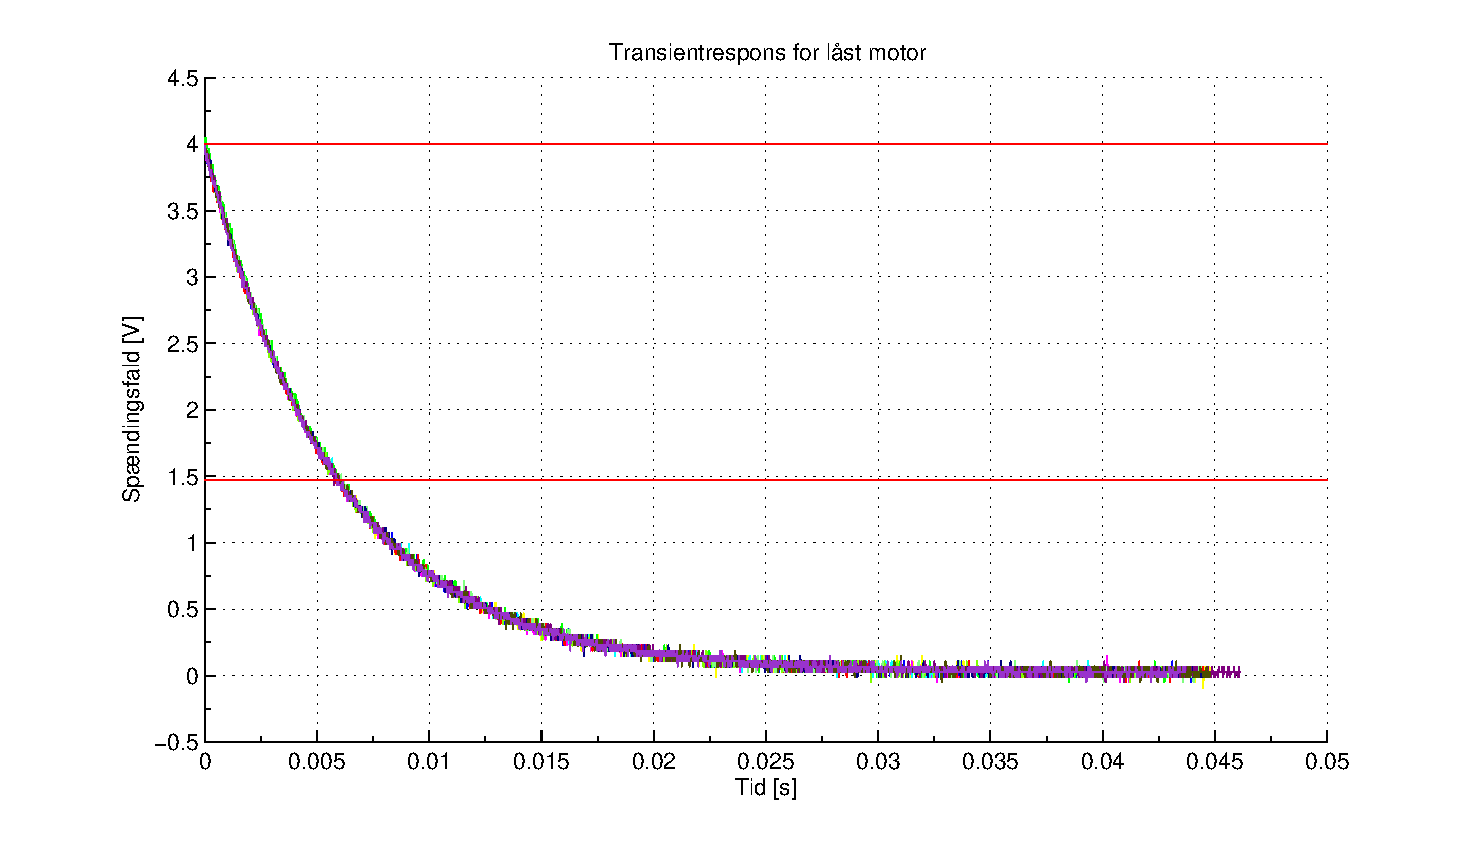
\includegraphics[width=1\textwidth]{./graphics/induktans0.eps}
	\caption[Transientrespons for låst motor]
		{Transientrespons for låst motor. De to vandrette røde linjer angiver spændingsniveauerne til bestemmelse af tidskonstanten.
		Den øverste linje er ved 4 [V], mens den nederste linje er ved \(4\cdot \frac{1}{e}\)  [V].}
	\label{fig:induktans0}
\end{figure}
Figur \ref{fig:induktans0} viser flere målingers transientrespons.

\paragraph{Metode 2\\}
Seriemodstanden \(R_{s1}\) er blevet målt til 473,3 \([\Omega]\).
Spændingen har en amplitude på 2,4 [V] og et DC-offset på 2,5 [V].
På figur \ref{fig:induktans1} er steady-state responsen for spændingsfaldene over DC-motoren og seriemodstanden indtegnet.
\begin{figure}[th!]
	\centering
	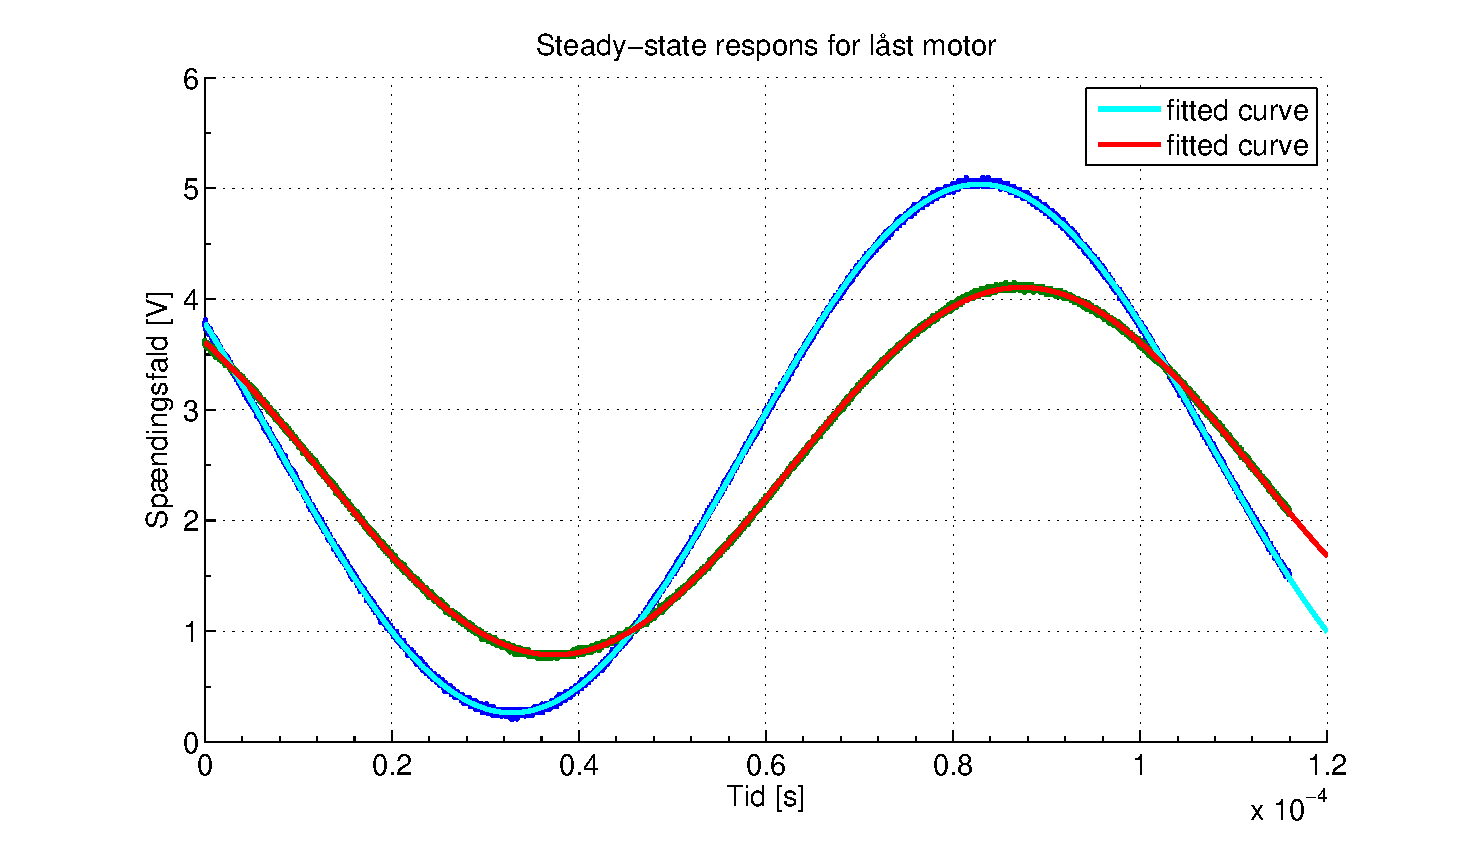
\includegraphics[width=1\textwidth]{./graphics/induktans1.eps}
	\caption[Steady-state respons for låst motor]
		{Steady-state respons for låst motor. Med mørkeblåt er markeret \(\mathbf{V_1}\) og med mørkegrønt \(\mathbf{V_2}\).
		To tilpassede sinuskurver, fundet vha. MATLAB's fit-funktion, er indtegnet med lyseblåt og rødt.}
	\label{fig:induktans1}
\end{figure}

\paragraph{Metode 3\\}
På figur \ref{fig:induktans2} er induktansmålingerne fra LCR-meteret indtegnet.
\begin{figure}[th!]
	\centering
	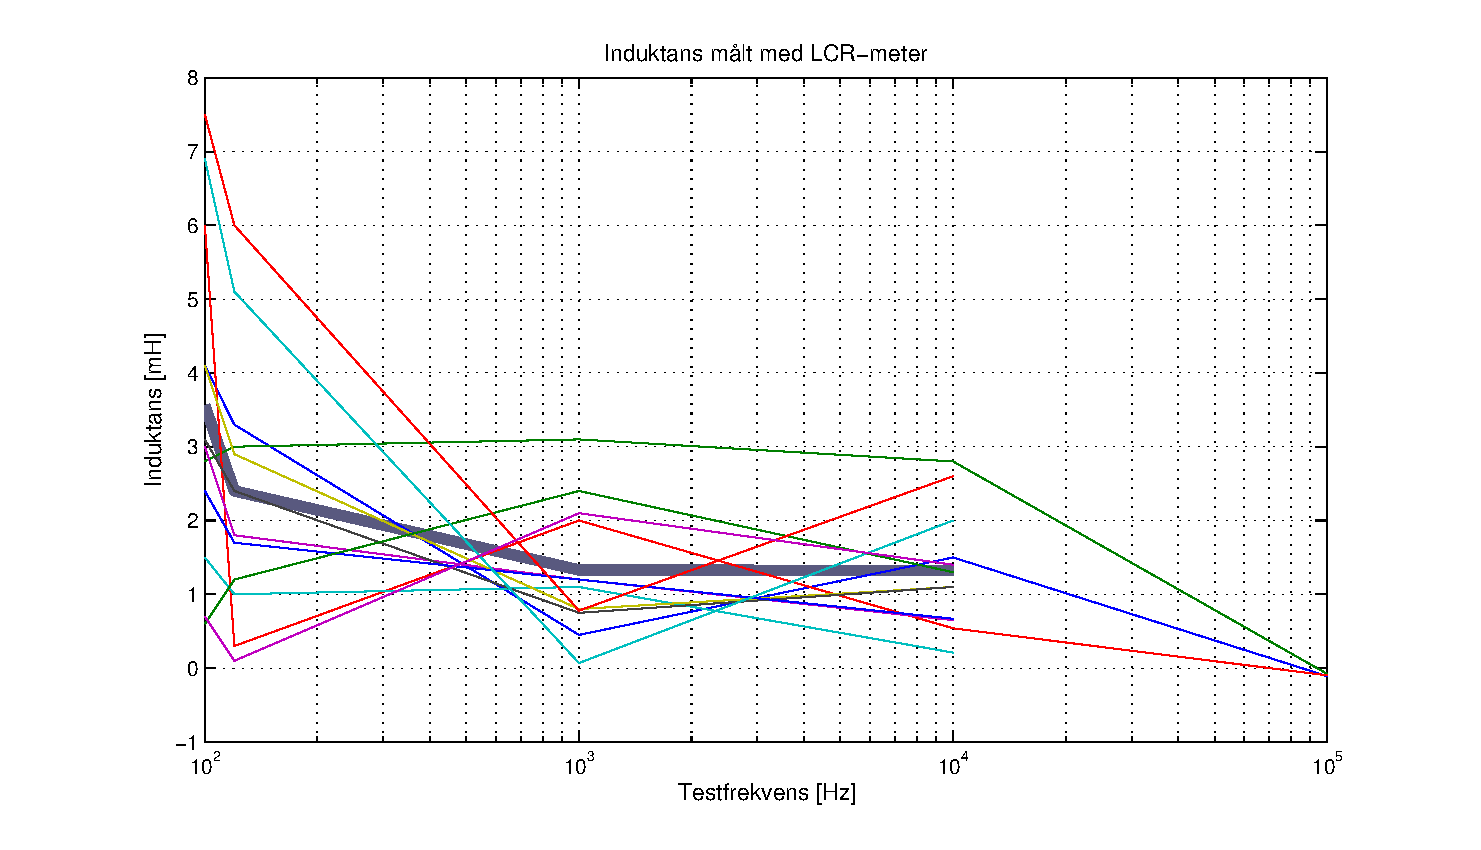
\includegraphics[width=1\textwidth]{./graphics/induktans2.eps}
	\caption[Induktans målt med LCR-meter]
		{Induktanser målt ved forskellige testfrekvenser og motorpositioner med LCR-meteret.
		For hver motorposition er der tegnet en linje gennem de 4-5 målepunkter.
		Ved 100 [kHz] er induktansen kun blevet målt for tre motorpositioner.
		Den tykke linje angiver gennemsnittet af de målte induktanser for de fire laveste testfrekvenser,
		100, 120, 1000 og 10000 [Hz].}
	\label{fig:induktans2}
\end{figure}

Det anvendte LCR-meter er af typen Agilent Techologies U1733C.

\subsubsection{Databehandling}
\paragraph{Metode 1\\}
For hver måling af transientresponsen, vist i figur \ref{fig:induktans0} er induktansen blevet
bestemt ved brug af ligning \ref{eq:induktans0}.
Gennemsnitsinduktansen er ved denne metode blevet fundet til \(L_m=0,395\) [H].

\paragraph{Metode 2\\}
Vha. MATLAB's fit-funktion er to sinuskurver blevet tilpasset til de målte spændingsfald.
Ud fra funktionsforskrifterne på de to sinuskurver er amplitudeforholdet \(\frac{A_1}{A_2}\)
og faseforskellen \(\phi\) blevet beregnet,
og vha. ligningerne \ref{eq:Rm_0} og \ref{eq:Lm_0} er resistansen hhv. induktansen blevet beregnet til
179,94 \([\Omega]\) hhv. 3,047 [mH].
Effektafsættelsen i motoren er med amplitudeforskellen på \(\mathbf{V_1}\) og \(\mathbf{V_2}\) samt
de i forsøget fundne værdier \(R_{s1}\) og \(R_m\) ved brug af ligning \ref{eq:effekt} beregnet til 0,405 [mW].

\paragraph{Metode 3\\}
Som det fremstår af figur \ref{fig:induktans2} er den målte induktans forskellig for hver testfrekvens.
Det blev fundet, at induktansmåling ved 100 [kHz] ikke var brugbar, da resultatet var negativt.
Derfor blev der kun foretaget tre målinger ved 100 [kHz].
For hver af de fire laveste testfrekvenser blev middelinduktansen fundet, og
en linje gennem disse induktanser er tegnet med fed på figur \ref{fig:induktans2}.

Gennemsnittet af de fire middelværdier er 2,2 [mH].

\subsubsection{Diskussion}
Den lineære sammenhæng mellem strøm og spænding fundet i afsnit \ref{ss:eksperiment1} kan ikke benægtes,
og for effektafsættelser i motoren på over 48 [mW] må resistansen kunne antages at være \(5,215\) \([\Omega]\)  som beregnet.
Men, som fundet ved forsøget med metode 2, så er motorens resistans langt højere,
179,94 \([\Omega]\) ved en effektafsættelse i motoren på 0,405 [mW].
Dette indikerer, at motorens ækvivalente resistans er lineær i de brugbare intervaller, altså ved de effektafsættelser en
praktisk applikation ville få brug for, altså over 48 [mW], men at motoren opfører sig anderledes når effektafsættelsen
bliver tilpas lille, i strørrelsesordenen under 1 [mW].
Til brug i modelleringen og simuleringen af motoren til den praktiske applikation, hvor motoren skal kunne rotere,
vurderes det derfor at den i afsnit \ref{ss:eksperiment1} fundne ækvivalente modstand på \(R_m=5,215\) \([\Omega]\) giver en meget nøjagtig værdi for den faktiske modstand i motoren.\\

Induktansen er imidlertid sværere at bestemme, da effektafsættelsen i de udførte forsøg er lav.
Resultatet fra metode 1 afviger meget fra resultaterne fra metode 2 og 3, og vurderes at være ubrugeligt
til modelleringen af motoren til den praktiske applikation.
I den praktiske applikation vil motoren blive udsat for en PWM-spænding med en PWM-frekvens på ca. 24 [kHz].
Denne PWM-spænding er er et skift mellem to DC-niveauer, og har en grundfrekvens på 24 [kHz].
Det vurderes derfor, at LCR-meterets resultater for 10 [kHz] danner det bedste grundlag for et
estimat af induktansen. Bemærk at den meget store spredning på målingerne på tværs af testfrekvenserne
gør, at estimatet kun er vejledende.
Der gives et vejledende estimat på 2,2 [mH].


\subsubsection{Konklusion}
Eksperiment 2 viser hvordan effektafsættelsen i DC motoren har betydning for dens resistans. Idet DC motorene i applikationen antages for at have en effektafsættelse over 48 [mW] medfører dette motorens har en resistans på \(R_m=5,215\) \([\Omega]\).\\

Til modelleringen af DC motoren estimeres motorens induktans til \(L_m\approx2.2\) \([mH]\).

\subsection{Eksperiment 3}
\label{ss:eksperiment3}
\subsubsection{Formål}
Bestemmelse af proportionalitetskonstanterne \(K_b\) og \(K_t\) samt den viskøse friktionskonstant \(B\).

\subsubsection{Teori}
Hvis man påfører motoren en DC-spænding og lader den rotere frit, uden ekstra belastning,
så kan ligning \ref{eq:Vm_transient1} omskrives til ligning \ref{eq:Vm_freerun0}.
\begin{equation}
	V_m=i_m\cdot{R_m}+K_b\cdot\omega
	\label{eq:Vm_freerun0}
 \end{equation}
Samtidig kan kraftmomentet udtrykkes ved ligning \ref{eq:Tm_leveret}, hvor det eneste inertimoment vil være
rotorens, navnlig \(J_m\).
Da vinkelhastigheden ikke ændrer sig ved steady-state kan ligningerne \ref{eq:Vm_freerun0} og \ref{eq:Tm_leveret} kombineres
til ligning \ref{eq:KtimBw}.
\begin{equation}
	K_t\cdot{i_m}=B\cdot\omega
	\label{eq:KtimBw}
 \end{equation}
Hvis man kender motorens ækvivalente modstand \(R_m\), steady-state strømmen \(i_m\) ved en steady-state spænding \(V_m\),
samt steady-state vinkelhastigheden \(\omega\), kan man altså vha. ligningerne \ref{eq:Vm_freerun0} og \ref{eq:KtimBw} bestemme
proportionalitetskonstanterne \(K_t\) og \(K_b\) (fordi de har samme numeriske værdi i SI-enheder) og friktionskonstanten \(B\).
\subsubsection{Fremgangsmåde}
Den ubelastede motor påføres en kendt DC-spænding, og motoren opnår steady-state.
Strømmen igennem motoren måles med et multimeter.
Vinkelhastigheden måles ved at tælle antallet af encoder-ticks på ét minut og kan omregnes til SI-enheder, 
idet det vides, at der er 360 ticks pr. omgang, \citep{emgmotor}.
For hver måling beregnes \(K_b\) og \(K_t\) samt \(B\) vha. ligningerne \ref{eq:Vm_freerun0} og \ref{eq:KtimBw}.

Det anvendte multimeter er af typen TTi 1604,
og antallet af ticks blev talt med en tæller på FPGA'en, der automatisk stopper efter 1 minut.
\subsubsection{Måleresultater}
I tabel \ref{tb:steadystatenoload} findes målingerne af strøm, spænding og vinkelhastighed.
\begin{figure}[th!]
	\centering
	\begin{tabular}{r|r|r}
$V_m$ [V]&$i_m$ [mA]&$\omega$ $\left[\frac{\text{ticks}}{\text{min}}\right]$\\\hline
12,00&97&76564\\ %12,000&97&76564
12,00&97&76741\\ %12,000&97&76741
10,01&96&62963\\ %10,007&96&62963
10,01&96&63379\\ %10,007&96&63379
8,584&92&54255\\
8,584&92&54374\\
7,154&90&44835\\
7,154&90&44089\\
6,000&89&36489\\
6,000&89&36224\\
\end{tabular}

	\captionsetup{type=table}
	\caption[Steady-state spænding, strøm og vinkelhastighed uden belastning]
			{Sammenhørende værdier af DC spænding over og strøm gennem, samt vinkelhastighed af motor uden belastning.}
	\label{tb:steadystatenoload}
\end{figure}
\subsubsection{Databehandling}
For hver måling er \(K_b\) og \(K_t\) samt \(B\) vha. ligningerne \ref{eq:Vm_freerun0} og \ref{eq:KtimBw} beregnet,
i SI-enheder. Til beregningen er anvendt den i afsnit \ref{ss:eksperiment1} fundne værdi for \(R_m\).
Gennemsnittet af hver parameter findes i tabel \ref{tb:kbktb}.
\begin{figure}[th!]
	\centering
	\begin{tabular}{r|r|r}
$K_b$ [$\text{V}\cdot\frac{\text{s}}{\text{rad}}$]&$K_t$ [$\frac{\text{N m}}{\text{A}}$]&$B$ [N m s]\\\hline
0,517&0,517&0,00319\\
\end{tabular}

	\captionsetup{type=table}
	\caption[Proportionalitetskonstanterne \(K_b\), \(K_t\) og \(B\)]
			{Proportionalitetskonstanterne \(K_b\), \(K_t\) og \(B\).}
	\label{tb:kbktb}
\end{figure}

\subsubsection{Diskussion}
De fundne værdier for \(K_b\), \(K_t\) og \(B\) vurderes at være nøjagtige approksimationer
til brug i modelleringen af systemet til en praktisk applikation, da de er fundet ved effektafsættelser
der afspejler effektafsættelser, der vil forekomme i applikationen.
Der er dog blevet set bort fra Coulomb-friktionen, og der vil skulle tages højde for dette under modelleringen.
\subsubsection{Konklusion}
Proportionalitetskonstanterne \(K_b\) og \(K_t\) er blevet fundet til i SI-enheder at have den numeriske værdi 0,517.
Den viskøse friktionskonstant \(B\) er blevet fundet til 0,00319 \([N \cdot m \cdot s]\).
Alle konstanterne er blevet fundet vha. værdien af \(R_m\) fra afsnit \ref{ss:eksperiment1}.
\subsection{Eksperiment 4}
\subsubsection{Formål}
Bestemmelse af rotorens inertimoment \(J_m\).
Bestemmelse af størrelsen på friktionen i motoren.
\subsubsection{Teori}
Hvis der ikke løber strøm igennem motoren,
kan ligning \ref{eq:Vm_transient1} omskrives til ligning \ref{eq:Vm_nocurrent}.
\begin{equation}
	V_m(t)=K_b\cdot\omega(t)
	\label{eq:Vm_nocurrent}
 \end{equation}

I dette forsøg fastgøres en masse til rotoren med en snor.
Massen lades falde til jorden med tyngdeaccelerationen.
Rotoren vil accelerere med vinkelaccelerationen \(\alpha_{op}\).
Jf. Newtons 2. lov vil det resulterende kraftmoment være givet ved ligning \ref{eq:Tres0}.
\begin{equation}
	T_{res}=J_m\cdot\alpha_{op}
	\label{eq:Tres0}
 \end{equation}
Dette kraftmoment kan også udtrykkes som kraftmomentet på rotoren fra snoren, \(T_{op}\),
fratrukket friktionskraftmomentet \(T_f\), som udtrykt i ligning \ref{eq:Tres1}.
\begin{equation}
	T_{res}=T_{op}-\left|T_f\right|
	\label{eq:Tres1}
 \end{equation}
Bemærk at \(T_f\) er hele friktionskraftmomentet, inkl. Coulomb-friktion.
Kraftmomentet \(T_{op}\) kan udtrykkes som rotorens radius \(r\) ganget med snorkraften, \(F_{snor}\),
som udtrykt i liginng \ref{eq:Top0}.
\begin{equation}
	T_{op}=r\cdot{F_{snor}}
	\label{eq:Top0}
 \end{equation}
Snorkraften kan udtrykkes ved tyngdekraften på massen samt den lineære acceleration af massen, \(a\),
som udtrykt i ligning \ref{eq:Fsnor0}, hvor a kan udtrykkes ved \(\alpha_{op}\) som i ligning \ref{eq:a}.
\begin{equation}
	F_{snor}=m\cdot(g-a)
	\label{eq:Fsnor0}
 \end{equation}
\begin{equation}
	a=r\cdot\alpha_{op}
	\label{eq:a}
 \end{equation}

Når rotoren har opnået en given vinkelhastighed, og snorkraften stopper,
vil rotoren decelerere med en vinkelacceleration \(\alpha_{ned}\), som skyldes friktionskraftmomentet,
jf. ligning \ref{eq:Tf0}.
\begin{equation}
	\left|T_f\right|=J_m\left|\alpha_{ned}\right|
	\label{eq:Tf0}
 \end{equation}

Inertimomentet \(J_{disk}\) for en disk (ring) med massen \(m_{disk}\), ydre radius \(r_{disk}\) og
indre radius \(r_{hul}\) er givet ved ligning \ref{eq:Jdisk},\citep[Side. 255, tabel 10-2b]{fund_of_physics}.
\begin{equation}
	J_{disk}=\frac{1}{2}\cdot{m_{disk}}\cdot\left(r_{hul}^2+r_{disk}^2\right)
	\label{eq:Jdisk}
 \end{equation}

Da rotorskaftet på DC-motoren ikke er cylinderformet, blev det valgt at montere en disk
på rotoren, således at de i teorien formler kan bruges til beregning af inertimomentet,
med diskens radius \(r_{disk}\).
Med ligningerne \ref{eq:Tres0}, \ref{eq:Tres1}, \ref{eq:Top0}, \ref{eq:Fsnor0}, \ref{eq:a}, \ref{eq:Tf0} samt \ref{eq:Jdisk}
kan rotorens inertimoment udtrykkes vha. de målbare størrelser
\(\alpha_{op}\), \(\alpha_{ned}\), \(m_{disk}\), \(r_{disk}\), \(r_{hul}\) og \(m_{lod}\) (massen af det fastgjorte lod),
mens friktionskraftmomentet kan udtrykkes vha. \(m_{lod}\), \(r_{disk}\), \(\alpha_{op}\) og \(\alpha_{ned}\),
som i ligningerne \ref{eq:Jrotor} og \ref{eq:Tf1}.
\begin{equation}
J_{ m }=m_{ lod }\cdot { r_{ disk } }\cdot \left| \frac { \alpha _{ op }\cdot { r_{ disk } }-g }{ \alpha _{ op }+\left| \alpha _{ ned } \right|  }  \right| -\frac { 1 }{ 2 } \cdot { m_{ disk } }\cdot \left( r_{ hul }^{ 2 }+r_{ disk }^{ 2 } \right) 
	\label{eq:Jrotor}
\end{equation}
\begin{equation}
\left| T_{ f } \right| =\alpha _{ ned }\cdot { m_{ lod } }\cdot { r_{ disk } }\cdot \left| \frac { \alpha _{ op }\cdot { r_{ disk } }-g }{ \alpha _{ op }+\left| \alpha _{ ned } \right|  }  \right| 
	\label{eq:Tf1}
 \end{equation}
\subsubsection{Fremgangsmåde}
En disk måles og vejes og monteres på rotorskaftet.
Et vejet lod fastgøres til disken med en snor, og snoren vikles rundt om disken.
Med et oscilloskop måles spændingsfaldet over motoren, mens loddet lades falde til gulvet.
Når loddet har ramt gulvet, og spændingsfaldet er 0 V, stoppes målingen, og forsøget gentages.
\subsubsection{Måleresultater}
Diksen har en masse på 21,2 [g], en ydre radius på 1,25 [cm] og en indre radius på 5 [mm].
Loddets masse er 851,7 [g].
På figur \ref{fig:vemf0} er målingerne af \(V_{EMF}\) indtegnet.

\begin{figure}[th!]
	\centering
	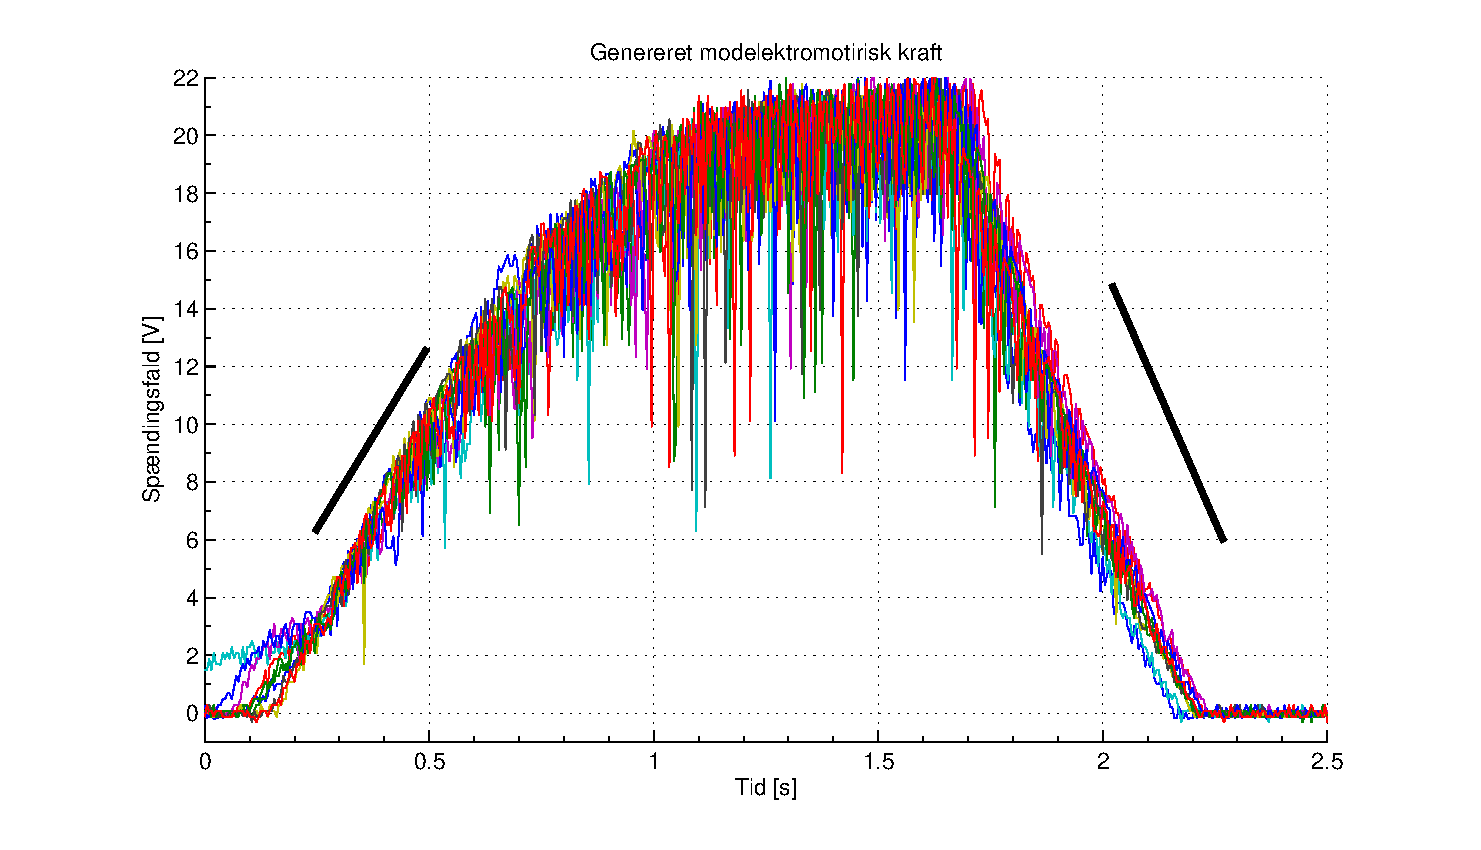
\includegraphics[width=1\textwidth]{./graphics/vemf0.eps}
	\caption[Målt modelektromotorisk kraft ved acceleration af motor]
		{Målt modelektromotorisk kraft ved acceleration af motor.
		De indtegnede sorte streger viser hældningerne før og efter loddet ramte jorden.
		På grafen vises målingerne fra flere forsøg sammen.}
	\label{fig:vemf0}
\end{figure}
\subsubsection{Databehandling}
Da målingerne er meget støjfyldte, valgtes det at lavpasfiltrere dem, så hældningsbestemmelsen
ikke bliver påvirket af den højfrekvente støj.
De lavpasfiltrerede data kan ses på figur \ref{fig:vemf1}.
\begin{figure}[th!]
	\centering
	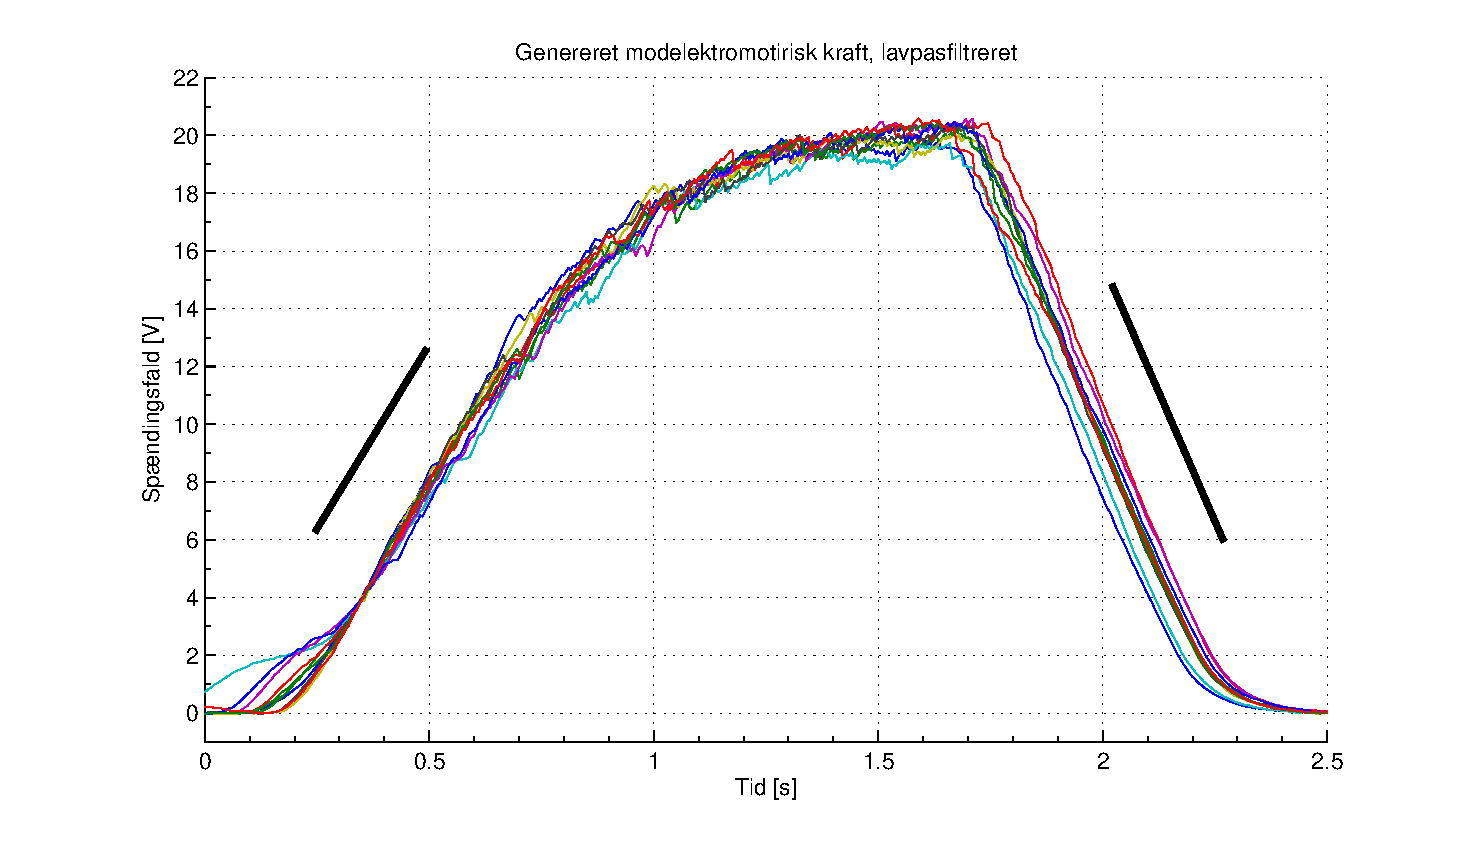
\includegraphics[width=1\textwidth]{./graphics/vemf1.eps}
	\caption[Målt modelektromotorisk kraft ved acceleration af motor, lavpasfiltreret]
		{Målt modelektromotorisk kraft ved acceleration af motor, lavpasfiltreret.
		De indtegnede sorte streger viser hældningerne før og efter loddet ramte jorden.
		På grafen vises målingerne fra flere forsøg sammen.}
	\label{fig:vemf1}
\end{figure}
Jf. ligning \ref{eq:Vm_nocurrent} er det målte spændingsfald proportionalt med
vinkelhastigheden, og hældningen af grafen vil således skulle divideres med \(K_b\),
før den repræsenterede vinkelaccelerationen. \(K_b\) blev bestemt i afsnit \ref{ss:eksperiment3}.
For hver måling bestemtes hældningerne \(\alpha_{op}\) og \(\alpha_{ned}\) vha. lineær regression på de lineære stykker,
og ud fra dette er gennemsnitsaccelerationerne blevet fundet til
\(\alpha_{op}=49,3\) \([\frac{\text{rad}}{\text{s}}]\) og \(\alpha_{ned}=-69,1\) \([\frac{\text{rad}}{\text{s}}]\).
Med disse værdier er inertimomentet beregnet vha. ligning \ref{eq:Jrotor}, og friktionskraftmomentet vha. ligning \ref{eq:Tf1}.
De beregnede værdier er hhv. \(J_m=8,26\cdot10^{-4}\) \([\text{kg}\cdot{\text{m}^2}]\) og \(\left| { T }_{ f } \right| =0,0571\) \( [\text{N} \cdot \text{m}]\).
\subsubsection{Diskussion}
At \(V_{EMF}\) aftager lineært fremfor eksponentielt indikerer,
at den viskøse friktion er lav i forhold til Coulomb-friktionen.
Den lineære approksimation der i fremgangsmåden benyttes er derfor anvendelig,
og giver et nøjagtigt billede af den tilstedeværende friktion samt rotorens inertimoment.
\subsubsection{Konklusion}
Rotorens inertimoment er bestemt til \(J_m=8,26\cdot10^{-4}\) \([\text{kg}\cdot{\text{m}^2}]\).
Friktionskraftmomentet er bestemt til \(\left| { T }_{ f } \right| =0,0571\) \( [\text{N} \cdot \text{m}]\).

\subsection{Opsummering af motorparameter}
\label{opsummering_af_motorparameter}
Nedenstående motorparameterne er fundet i Eksperiment 1-4 og disse værdier bruges til modelering af DC motorene.
\begin{itemize}
\item \(R_m\)=5,215 \([\Omega]\)
\item \(L_m = 3,047\) \([mH]\) \todo{update value}
\item \(K_b = 0,517\) \(\left[ V\cdot\frac{s}{rad} \right] \)
\item \(K_t = 0,517\) \(\left[ \frac{N\cdot m}{A} \right] \)
\item \(B = 0,00319\) \(\left[  N \cdot m \cdot s\right]  \)
\item \(J_m = 8,26\cdot10^{-4}\) \(\left[ kg\cdot{m^2} \right]  \)
\item \(\left| T _f \right| = 0,0571\) \(\left[ N \cdot m \right]   \)
\end{itemize}